\documentclass[a4paper,12pt,titlepage]{article}
\usepackage[a4paper]{geometry}
\usepackage[ngerman]{babel}
\usepackage{fontspec}
\setmainfont[Ligatures=TeX]{Linux Libertine O}
\usepackage{csquotes}
\usepackage{hyperref}
% \usepackage{graphicx}
\title{Hamelner Party-Broker Warenwirtschaftssystem}
\author{Florian Bussmann \and Leon Westhof \and Jona Stubbe}
\begin{document}
% \frontmatter
\maketitle
\tableofcontents

\part{Programmentwurf}
\section{Klassendiagramm}
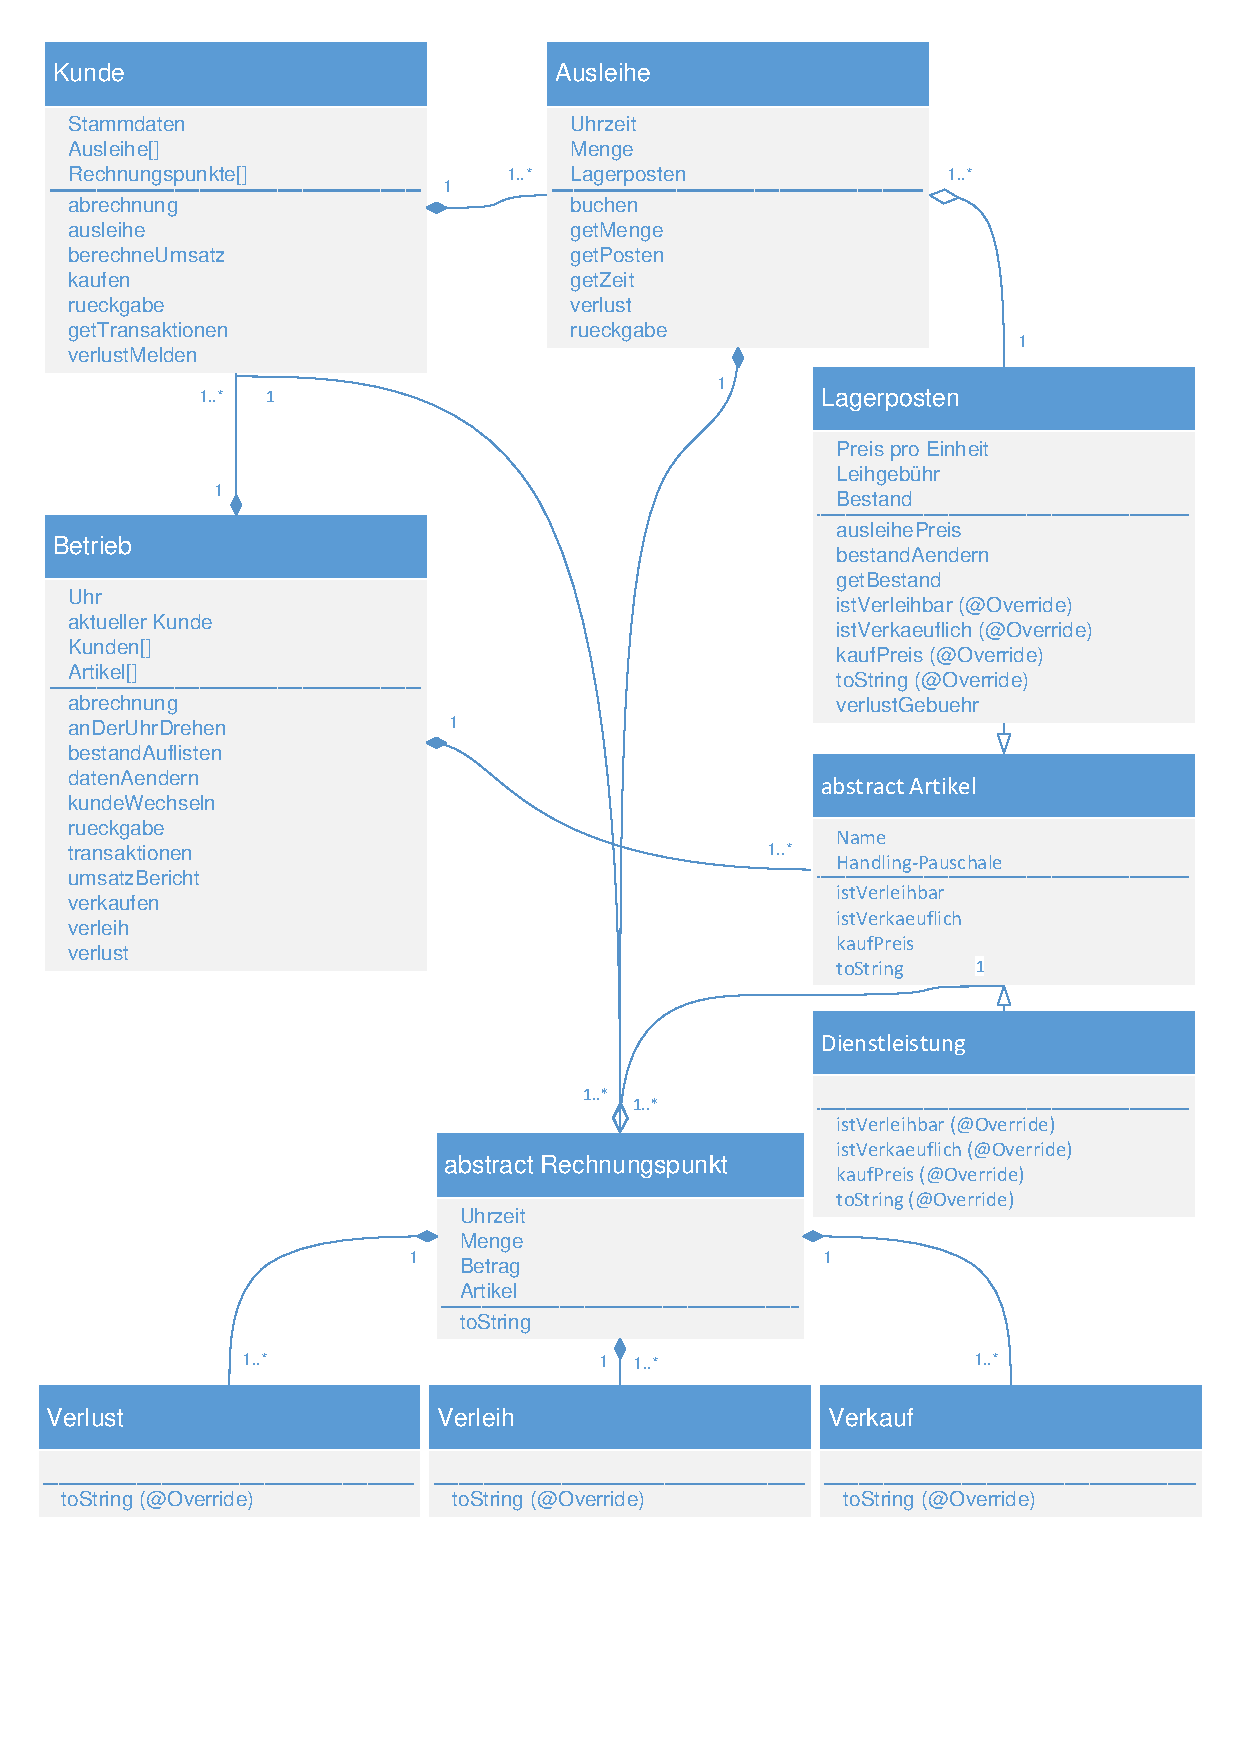
\includegraphics[width=\textwidth]{Klassendiagramm.pdf}
\newpage
\section{Funktionsumfang}
Befehle zur / zum:
\begin{enumerate}
\item Auflistung der aktuell verfügbaren verkäuflichen Gegenstände
\item Auflistung der aktuell verfügbaren  Leihgegenstände
\item Auflistung des gesamten verkäuflichen und verleihbaren Bestands
\item Auflistung der aller Kunden mit ihren Gesamtumsätzen
\item Auflistung aller offenen Transaktionen  und fertigen rechnungspunkte eines Kunden
\item Verkauf eines verfügbaren Objekts
\item Ausleihe eines verfügbaren Objekts für eine prognostizierte Zeitdauer
\item Rückgabe einer vollständigen oder unvollständigen Menge an Objekten
\item Verlustmeldung eines Teiles bzw. der gesamten Ausleihe
\item Abrechnung eines Kunden bei  Rückgabe, Verlust, Kauf oder Nutzung einer Dienstleistung für die entsprechenden Mengen (keine Berücksichtigung von noch ausgeliehenen Gegenständen)
\item Anlegen und Ändern von Kundendaten
\item Wechsel zwischen Kunden
\end{enumerate}
\section{Methodenbeschreibung}
\subsection{Kunde}
\begin{description}
\item[\{set, get\}\{Name, VorName, ID, Straße, Hausnummer, PLZ, Ort\}]
Holt oder ändert die entsprechenden Werte.
\item[rueckgabe(posten, zeit, menge) -> Verleih]
Bucht eine gegebene Menge eines gegebenen Postens von den Ausleihen des Kunden zurück ins Lager
und stellt die Kosten der Ausleihe dem Kunden in Rechnung.\\
Exception wenn der Posten nicht ausgeliehen war oder die angegebene Menge die Leihmenge übersteigt.
\item[verlustMelden(posten, zeit, menge) -> Verlust]
Streicht eine gegebene Menge eines gegebenen Postens von den Ausleihen des Kunden\\
Exception wenn der Posten nicht ausgeliehen war oder die angegebene Menge die Leihmenge übersteigt.
und stellt dem Kunden die Verlustgebühr in Rechnung.
\item[ausleihe(ausleihe)]
Fügt eine Ausleihe dem Kundenkonto hinzu. Dabei wird diese gebucht.
\item[abrechnung(zeit) $\rightarrow$ RechnungPosten{[]}]
Gibt alle ausstehenden Rechnungspunkte zurück und legt sie damit zu den bearbeiteten Rechnungspunkten.
\item[berechneUmsatz() $\rightarrow$ geld]
Berechnet den gesamten Umsatz, der durch den Kunden verursacht wurde, d. h. der Wert aller bearbeiteten Rechnungspunkte.
\item[getTransaktionen() $\rightarrow$ String{[]}]
Stellt alle Rechungspunkte und bestehenden Ausleihen zusammen.
\item[kaufen(artikel, menge, zeit)]
Verkauft (entfernt Bestand) und stellt dem Kunden den Kaufpreis in Rechnung.
\end{description}
\subsection{Ausleihe}
\begin{description}
\item[buchen()]
Die Ausleihe tritt in Kraft: Entfernt die auszuleihende Menge des Posten aus dem Lager.
\item[getPosten() $\rightarrow$ LagerPosten]
Gibt den Posten der geliehen wird, zurück.
\item[getMenge() $\rightarrow$ menge]
Gibt die ausgeliehende / auszuleihende Menge zurück.
\item[getZeit() $\rightarrow$ zeit]
Gibt die Startzeit der Ausleihe zurück.
\item[reduzieren(menge) $\rightarrow$ Ausleihe]
Annuliert eine bestimmte Menge in der Ausleihe, gibt geänderte Ausleihe zurück.
\end{description}
\subsection{Artikel (abstract)}
\begin{description}
\item[toString() $\rightarrow$ String]
gibt den Namen des Artikels zurück
\item[bestandString() $\rightarrow$ String]
die Daten des Postens, zB in der Form \enquote{<Bestand> x <ID> <Name> (<Preise>)} als String zurück
\item[istVerkaeuflich() $\rightarrow$ boolean]
Bestimmt ob der Artikel verkäuflich ist.
\item[istVerleihbar() $\rightarrow$ boolean]
Bestimmt ob der Artikel verleihbar ist.
\item[kaufPreis(menge) $\rightarrow$ geld]
Bestimmt den Kaufpreis einer gegebenen Menge des Postens.
\end{description}
\subsection{Lagerposten}
\begin{description}
\item[bestandAendern(menge)]
Ändert den Bestand um die angegebene Menge (positiv oder negativ). \\
Exception wenn Bestand negativ werden würde.
\item[getBestand() $\rightarrow$ geld]
Gibt den aktuellen Lagerbestand zurück.
\item[ausleihePreis(zeit, menge, zeitDelta) $\rightarrow$ geld]
Bestimmt die Leihgebühr einer gegebenen Menge des Postens über eine gegebene Zeitspanne.
\item[verlustGebuehr(zeit, menge, zeitDelta) $\rightarrow$ geld]
Bestimmt die Gebühr, die bei Verlust einer gegebenen Menge des Postens nach gegebener Zeit entsteht.

\end{description}
\subsection{Betrieb}
\begin{description}
\item[main(args)]
Hauptmenü
\item[bestandAuflisten(modus)]
listet den Bestand, gefiltert nach Kriterien, die durch modus bestimmt werden (Gesamtbestand, verf. Verkaufsware, verf. Verleihware, oÄ), auf
\item[verkaufen()]
der Verkaufs-Menüpunkt
\item[verleih()]
der Verleih-Menüpunkt
\item[abrechnung()]
rechnet alle ausstehenden Rechnungspunkte beim aktuellen Kunden ab
\item[rueckgabe()]
der Rückgabe-Menüpunkt
\item[verlust()]
der Verlust-Meldungs-Menüpunkt
\item[umsatzBericht()]
listet die Umsätze der Kunden auf
\item[datenAendern()]
ändert die Daten des aktuellen Kunden (Untermenü)
\item[transaktionen()]
zeigt die Transaktionen des aktuellen Kunden an
\item[anDerUhrDrehen(zeit)]
schreitet die Zeit voran
\item[kundeWechseln()]
wechselt den aktiven Kunden
\end{description}
\section{Testfälle}
\begin{enumerate}
\item
Auflistung des Gesamtbestandes zum Kaufen und zum Verleihen.\\
$\Rightarrow$ Liste mit n Elementen zum Verkaufen und n Elementen zum Verleihen
\item
Auflistung des Gesamtbestandes zum Kaufen und zum Verleihen nach einer Änderung um x.\\
$\Rightarrow$ Liste mit n-x bzw. n+x Elementen zum Verkaufen und zum Verleihen
\item
Auflistung des aktuell verfügbaren Bestandes zum Ausleihen und zum Kaufen.
$\Rightarrow$ Liste mit y Elemente unterschiedlich(nach Ausleihe oder Verkauf) bzw. gleich zur Liste des Gesamtbestandes.
\item
Auflistung des aktuell verfügbaren Bestandes zum Ausleihen und zum Kaufen nach einer Ausleihe bzw. eines Kaufe.
$\Rightarrow$ Liste mit y Elemente unterschiedlich(nach Ausleihe oder Verkauf) bzw. gleich zur Liste des Gesamtbestandes.
\item
Verleihen von verfügbaren, nicht verfügbaren (die größer sind als die verfügbaren Mengen) und nichtganzzahligen Mengen.
$\Rightarrow$ Führt zu Veränderungen am Bestand der zurzeit verfügbaren Objekten, sofern es verfügbar war
\item
Verkauf von verfügbaren, nicht verfügbaren (die größer sind als die verfügbaren Mengen) und nichtganzzahligen Mengen.
$\Rightarrow$ Führt zu Veränderungen am Gesamtbestand und am zurzeit verfügbaren Bestand, sofern es verfügbar war
\item
Rückgabe von Mengen, die die Ausleihe übersteigen(sollte nicht möglich sein).
$\Rightarrow$ sollte eine Fehlermeldung ausgeben und keine Ausleihmengen, Rechnungspunkte oder sonstige Daten ändern
\item
Rückgabe testen:
\begin{itemize}
\item vollständig
\item unvollständig
\item im teilweise oder vollständigen Verlustfall
\end{itemize}
$\Rightarrow$ Veränderungen der Liste aktuell verfügbarer Objekte, macht eine Abrechnung , löscht oder ändert(bei unvollständig) das entsprechende Ausleih-Objekt und den Verweis
\item
Abrechnung testen.
$\Rightarrow$ schafft einen neuen Rechnungspunkt mit den Daten von Objekt Menge, Zeitraum und Kosten
\item
Umsatzliste testen.
$\Rightarrow$ Gibt eine Liste mit einem Eintrag pro Kunden aus, wo die Gesamtsumme der Transaktionen steht
\item
Transaktionen auflisten.
$\Rightarrow$ Gibt eine Liste von n Rechnungspunkten mit Menge, Art, Zeitraum, Preis der Transaktion und Gesamttransaktionenpreis für einen bestimmten Kunden aus
\item
Kundendaten ändern
$\Rightarrow$ Sollte die entsprechende Änderung speichern und zurückgeben
\item
Neuen Kunden aufnehmen.
$\Rightarrow$ erzeugt ein neues Kundenobjekte, führt zu einem weiteren Eintrag in der Umsatzanzeige
\item
Computer-Mensch Dialog überprüfen (auf Aktionen die möglich sind und welche die nicht möglich sind).
$\Rightarrow$ Fehlermeldungen bei Falscheingabe
\item
Kauf von nicht verkäuflichen Objekten(sollte nicht möglich sein).
$\Rightarrow$ Fehlermeldungen bei Falscheingabe, keine Änderung von Daten(Gesamtbestand, zurzeit verfügbarer Bestand, Rechnungspunkt )
\item
Leih von von nicht verleihbaren Objekten(sollte nicht möglich sein).
$\Rightarrow$ Fehlermeldungen bei Falscheingabe, keine Änderung von Daten(zurzeit verfügbarer Bestand, Ausleihobjekt )
\item
Zeitpunkt in die Vergangenheit ändern bzw. negative Zeitdauer(sollte nicht möglich sein).
$\Rightarrow$ Fehlermeldung, keine Datenänerung, bitte um Neueingabe
\item
Zeitpunkt in die Zukunft ändern.
\item
Differenzberechnung zwischen entliehenem und zurückgegebenen Zeitpunkt
\item
Kunden wechseln
$\Rightarrow$ Gibt eine entsprechende Meldung aus und übergibt einen anderen KundenID-Wert an die Methoden
\item
Programm unterscheidet zwischen Gegenständen und Dienstleistungen
$\Rightarrow$ Bei Dienstleistungen werden keine Änderungen des Gesamt- oder zuzeitverfügbaren Bestandes durchgeführt, keine Verlustpaschale, Leihgebür oder verkaufsgebür  berechnet und in den Rechnungsposten aufgenommen
\item Überprüfung der Berücksichtigung der Handlingpauschale
$\Rightarrow$ handlingpauschale wird bei Verkauf und Verleih bei Rückgabe pro Objekt mitberücksichtigt und in den Rechnungsposten mitaufgenommen, bei Verlust hingegen nicht
\item Toilettenwagen und Frischwasser können nicht verlohren werden
\item Dienstleistungen werden vorher als Rechnungspunkt berechnet
\end{enumerate}


\renewcommand\enquote[1]{{\ttfamily \bfseries #1}}

\part{Benutzerhandbuch}
\section{Der Startbildschirm}
Nach dem Programmstart sehen Sie in der Ausgabe \enquote{Kunde Mertens, Robert erfolgreich erstellt. Seine ID ist 1.}.
Diese Standartmeldung sagt Ihnen, dass ein Kunde mit der Kunden-ID 1 und dem Namen Robert Mertens erstellt wurde.

In der zweiten Zeile steht \enquote{Für Befehlsliste 0 eingeben}.
Dieser Hinweis sagt Ihnen, dass Sie in der Befehlszeile die 0 für die Liste aller möglichen Befehle eingeben können.
Sie können als vorgebildeter Nutzer aber auch jede andere Nummer, die sich von anderen Nutzungen her kennen, eingeben.

Nachdem Sie die 0 eingegeben haben, sehen Sie in den ersten 3 Zeilen den aktuellen Kunden mit dem Sie nun arbeiten.
Sollte dieser nicht neben Ihnen am Arbeitstisch sitzen oder Sie jemand anderen Bearbeiten wollen, lesen Sie im Kapitel Kunden wechseln nach wie das geht.

\section{Die Befehle}
Jeden eingegebenen Befehl müssen Sie mit Enter bestätigen.

\subsection{Der Status}
Mit dem Befehl 0 erhalten Sie einige Zeilen, die den aktuell ausgewählten Kunden und dessen Kundendaten beschreiben,
gefolgt von der Befehlsliste.

\subsection{Liste aller zur Zeit verkäuflichen Objekte}
Mit 1 können Sie im ersten Teil alle Objekte sehen,
 die einerseits verkäuflich sind und andererseits zur Zeit verfügbar (im Lager) sind und im zweiten Teil der Liste sehen Sie alle Dienstleistungen.

In der ersten Zeile sehen Sie die Meldung \enquote{Auflistung der aktuell verfügbaren verkäuflichen Gegenstände}
 und in der Zweiten die Überschriften der folgenden Tabelle: ID und Artikel.
Vor den Objekten sehen Sie die ID der Objekte, welche immer gleich ist
 und dieses Objekt kennzeichnet.
Damit können Sie in weiteren Funktionen diese Objektgruppe auswählen,
 jedoch erhalten Sie immer auch eine Liste mit den Objekten auf welche Sie diese Funktionen anwenden können.

Dahinter sehen Sie die aktuelle verfügbare Menge an Objekten und dahinter den Namen des Objektes.
Hinter den Namen sehen Sie in Klammern die entsprechenden Kosten für die Objekte.
Bei Objekten sehen Sie zuerst den Kaufpreis, dann die Handlinggebühr und die tägliche Leihgebühr.
Dienstleistungen können Sie an dem unterschiedlichen Formatierungsstil erkennen:
Bei diesen stehen die Kosten für eine Nutzung der Dienstleistung einfach dahinter.
Danach springt das Programm wider in das Hauptmenü.
\subsection{Liste aller zur Zeit verleihbaren Gegenstände}
Mit 2 in der Eingabezeile können Sie alle Objekte sehen,
 die einerseits verleihbar sind und andererseits zur zeit verfügbar, also im Lager sind.

In der ersten Zeile sehen Sie die Meldung \enquote{Auflistung der aktuell verfügbaren verkäuflichen Gegenstände}
 und in der Zweiten die Überschriften der folgenden Tabelle: ID und Artikel.
Vor den Objekten sehen Sie die ID der Objekte, welche immer gleich ist und dieses Objekt kennzeichnet.
Damit können Sie in weiteren Funktionen diese Objektgruppe auswählen,
 jedoch erhalten Sie immer auch eine Liste mit den Objekten auf welche Sie diese Funktionen anwenden können.

Dahinter sehen Sie die aktuelle verfügbare Menge an Objekten und dahinter den Namen des Objektes.
Hinter den Namen sehen Sie in Klammern, die entsprechenden Kosten für die Objekte.
Bei Objekten, die sowohl verleihbar als auch verkäufliche sind sehen Sie zuerst den Kaufpreis.
Diese ist hier nicht von Bedeutung.
Danach -- oder bei Objekten, die nur die nur verleihbar sind, am Anfang --
steht die Handlinggebühr und die tägliche Leihgebühr.
Danach springt das Programm wider in das Hauptmenü.

\subsection{Auflistung des verkäuflichen Gesamtbestandes}
Mit dieser Option, welche Sie mit 3 aufrufen, sehen Sie den Bestand an Objekten, die verkäuflich sind.
In der ersten Zeile sehen Sie die Meldung \enquote{Auflistung des gesamten verkäuflichen Bestands}
 und in der Zweiten die Überschriften der folgenden Tabelle: ID und Artikel.

Folgend sehen Sie nun die schon bekannte Objekt-ID und den entsprechenden Artikel.
Danach springt das Programm wider in das Hauptmenü.
\subsection{Verkauf eines Objektes}
Mit 4 öffnen Sie einen Menüpunkt zum Verkaufen eines Objektes bzw. zum Buchen einer Dienstleistung.
Seien Sie noch mal daraufhin gewiesen, dass alle Aktionen mit dem ausgewählten Konto durchgeführt werden.

In der ersten Zeile sehen Sie die Meldung \enquote{Verkauf eines verfügbaren Objekts}
 und in der Zweiten die Meldung \enquote{Zum Verkauf stehen derzeit folgende Produkte zur Verfügung:}.
Danach folgen die Überschriften der folgenden Tabelle: ID und Artikel.

Vor den Objekten sehen Sie die ID der Objekte, welche immer gleich ist und dieses Objekt kennzeichnet.
Damit können Sie in weiteren Funktionen diese Objektgruppe auswählen,
 jedoch erhalten Sie immer auch eine Liste mit den Objekten auf welche Sie diese Funktionen anwenden können.

Dahinter sehen Sie die aktuell verfügbare Menge an Objekten und dahinter den Namen des Objektes.
Hinter den Namen sehen Sie in Klammern, die entsprechenden Kosten für die Objekte.
Bei Objekten, die sowohl verleihbar als auch verkäufliche sind sehen Sie zuerst den Kaufpreis.
Danach -- oder bei Objekten, die nur die nur verleihbar sind, am Anfang --
steht die Handlinggebühr und die tägliche Leihgebühr.

In der letzten Zeile sehen Sie die Meldung \enquote{Welches Produkt möchten Sie verkaufen?}.
Dahinter schreiben Sie einfach die Produkt-ID. Bei einer Falscheingabe erhalten Sie die Meldung \enquote{Produktnummer ungültig.}.
Nachdem Sie nun ein Objekt gewählt haben,
 erhalten Sie bei Objekten eine Auskunft über die verfügbare Menge und in Klammer die Kosten.

Danach werden Sie nach der Menge gefragt, die Sie ausleihen möchten.
Bei Dienstleistungen werden Sie gefragt wie viele Sie benötigen.
Nach der Eingabe erhalten Sie eine Zusammenfassung des Gewählten mit Kosten. 
Diese können Sie nun mit j bestätigen, wobei Sie eine Bestätigung der Buchung erhalten oder Abbrechen,
 wobei die Meldung \enquote{Verkauf abgebrochen.} ausgegeben wird.
Danach springt das Programm wider in das Hauptmenü.

\subsection{verleihbarer Gesamtbestand}
Mit dieser Option, welche Sie mit 5 aufrufen, sehen Sie den Bestand an Objekten,
 die verkäuflich sind und alle angebotenen Dienstleistungen.

In der ersten Zeile sehen Sie die Meldung \enquote{Auflistung des gesamten verkäuflichen Bestands}
 und in der Zweiten die Überschriften der folgenden Tabelle: ID und Artikel.
Folgend sehen Sie nun die schon bekannte Objekt-ID und den entsprechenden Artikel.
Danach springt das Programm wider in das Hauptmenü.

\subsection{Ausleihe}
Mit 6 öffnen Sie den Menüpunkt zum Verleihen eines Objektes.
Seien Sie noch mal daraufhin gewiesen, dass alle Aktionen mit dem ausgewählten Konto durchgeführt werden.

In der ersten Zeile sehen Sie die Meldung \enquote{Ausleihe eines verfügbaren Objekts für eine prognostizierte Zeitdauer}
 und in der Zweiten die Meldung \enquote{Zum Verleih stehen derzeit folgende Produkte zur Verfügung:}.
Danach folgen die Überschriften der folgenden Tabelle: ID und Artikel.
Vor den Objekten sehen Sie die ID der Objekte, welche immer gleich ist und Objekt kennzeichnet. 
Dahinter sehen Sie die aktuelle verfügbare Menge an Objekten und dahinter den Namen des Objektes.

Hinter den Namen sehen Sie in Klammern, die entsprechenden Kosten für die Objekte.
Bei Objekten sehen Sie zuerst den Kaufpreis, dann die Handlinggebühr und die tägliche Leihgebühr.

In der letzten Zeile sehen Sie die Meldung \enquote{Welches Produkt möchten Sie verkaufen?}.
Dahinter schreiben Sie einfach die Produkt-ID.
Bei einer Falscheingabe erhalten Sie die Meldung \enquote{Produktnummer ungültig.}.
Nachdem Sie nun ein Objekt gewählt haben,
 erhalten Sie bei Objekten eine Auskunft über die verfügbare Menge und in Klammer die Kosten.
Danach werden Sie nach der Menge gefragt, die Sie ausleihen möchten und abschließend nach der Ausleihdauern in Tagen.
Nach dieser Eingabe erhalten Sie eine Zusammenfassung des Gewählten mit Kosten.

Diese können Sie nun mit j bestätigen, wobei Sie eine Bestätigung der Buchung erhalten oder Abbrechen,
 wobei die Meldung \enquote{Verkauf abgebrochen.} ausgegeben wird.
Danach springt das Programm wider in das Hauptmenü.
\subsection{Rückgabe eines Objektes}
Mit 7 können Sie Objekte zurückgeben.
Seien Sie noch mal daraufhin gewiesen, dass alle Aktionen mit dem ausgewählten Konto durchgeführt werden.

In der ersten Zeile sehen Sie die Meldung \enquote{Rückgabe eines entliehenen Objekts}
 und in der Zweiten die Überschriften der folgenden Tabelle: ID und Artikel.
Vor den Objekten sehen Sie die ID der Objekte, welche immer gleich ist und dieses Objekt kennzeichnet.
Damit können Sie in weiteren Funktionen diese Objektgruppe auswählen,
 jedoch erhalten Sie immer auch eine Liste mit den Objekten auf welche Sie diese Funktionen anwenden können.
Dahinter sehen Sie die aktuelle verfügbare Menge an Objekten und dahinter den Namen des Objektes.
Hinter den Namen sehen Sie in Klammern, die entsprechenden Kosten für die Objekte.
Bei Objekten sehen Sie zuerst den Kaufpreis, dann die Handlinggebühr und die tägliche Leihgebühr.

Nachdem Sie eines ausgewählt haben oder bei Falscheingabe zur erneuten Eingabe aufgefordert werden,
 werden Sie gebeten die Rückgabemenge anzugeben.
Bei Falscheingabe werden Sie auch hier wieder zu einer erneuten Eingabe aufgefordert.
Auf Mengenfehler werden Sie jedoch erst nach der Bestätigung hingewiesen.
In einem solchen Fall wird der Vorgang mit Fehlermeldung abgebrochen.
Ihre Eingabe können Sie nun mit j bestätigen,
 wobei Sie eine Bestätigung der Buchung erhalten oder Abbrechen,
 wobei die Meldung \enquote{Verkauf abgebrochen.} ausgegeben wird.
Danach springt das Programm wider in das Hauptmenü.
\subsection{Verlustmeldung}
Mit 8 können Sie Verluste melden.
Seien Sie noch mal daraufhin gewiesen, dass alle Aktionen mit dem ausgewählten Konto durchgeführt werden.

In der ersten Zeile sehen Sie die Meldung \enquote{Verlustmeldung eines entliehenen Objekts}
 und in der Zweiten die Überschriften der folgenden Tabelle: ID und Artikel.
Vor den Objekten sehen Sie die ID der Objekte, welche immer gleich ist und dieses Objekt kennzeichnet.
Damit können Sie in weiteren Funktionen diese Objektgruppe auswählen,
jedoch erhalten Sie immer auch eine Liste mit den Objekten auf welche Sie diese Funktionen anwenden können.
Dahinter sehen Sie die aktuelle verfügbare Menge an Objekten und dahinter den Namen des Objektes.
Hinter den Namen sehen Sie in Klammern, die entsprechenden Kosten für die Objekte.
Bei Objekten sehen Sie zuerst den Kaufpreis, dann die Handlinggebühr und die tägliche Leihgebühr.

Nachdem Sie eines ausgewählt haben oder bei Falscheingabe zur erneuten Eingabe aufgefordert werden,
 werden Sie gebeten die Verlustmenge anzugeben.
Bei Falscheingabe werden Sie auch hier wieder zu einer erneuten Eingabe aufgefordert.
Auf Mengenfehler werden Sie jedoch erst nach der Bestätigung hingewiesen.
In einem solchen Fall wird der Vorgang mit Fehlermeldung abgebrochen.
Ihre Eingabe können Sie nun mit j bestätigen, wobei Sie eine Bestätigung der Buchung erhalten oder Abbrechen,
 wobei die Meldung \enquote{Verkauf abgebrochen.} ausgegeben wird.
Danach springt das Programm wider in das Hauptmenü.
\subsection{Abrechnungen}
Mit dieser Methode, welche mit 9 aufgerufen wird, können Sie die letzten Aktionen des Kunden abrechnen.
In der ersten Zeile sehen Sie die Meldung \enquote{Abrechnung des aktuellen Kunden} und danach die entsprechenden Abrechnungen.
Danach springt das Programm wieder in das Hauptmenü.

\subsection{Transaktionen aller Kunden}
Mit 10 wird Ihnen eine Liste gezeigt in der alle Kunden mit Ihren Gesamtumsatz aufgelistet werden.
In der ersten Zeile sehen Sie die Meldung \enquote{Auflistung aller Kunden mit ihren Umsätzen}.
Folgend sehen Sie alle Kunden beginnend mit Ihrer Kunden-ID, danach ihrem Namen und ihrem Gesamtumsatz.
Danach springt das Programm wider in das Hauptmenü.
\subsection{Transaktionen eines Kunden}
Mit dieser Methode, welche mit 11 aufgerufen wird, können Sie alle Transaktionen des Kunden sehen.
In der ersten Zeile sehen Sie die Meldung \enquote{Auflistung der mit dem aktuellen Kunden durchgeführten Transaktionen}
 und danach die entsprechenden Abrechnungen.
Danach springt das Programm wider in das Hauptmenü.
\subsection{Neuen Kunden Anlegen}
Mit 12 können Sie einen neuen Kunde anlegen.
Sie werden in Folge nach den folgenden Angaben gefragt: Nachnamen, Vornamen, Straße, Hausnummer, Postleitzahl, Ort.
Abschließend erhalten Sie eine Meldung über den angelegten Kunden und die zugewiesene ID.
Achtung: Es wurde nun automatisch der aktive Kunde auf den Neuen gewechselt.
Danach springt das Programm wider in das Hauptmenü.
\subsection{Kundendaten ändern}
Mit dieser Option, welche Sie mit 13 aufrufen, können Sie bestimmte Kundendaten ändern.

Sofern Sie 1 wählen können Sie die komplette Anschrift ändern.
Dabei werden Sie in Folge nach Ort, Postleitzahl, Straße und Hausnummer gefragt.
Bei Nummerfalscheingaben erhalten Sie eine Fehlermeldung und werden zur Neueingabe aller Parameter aufgefordert.

Wenn Sie 2 gewählt haben, können Sie die Hausnummer und Straße ändern.
Dafür werden Sie zur Eingabe der Straße und dann der Hausnummer gefragt.
Bei Nummerfalscheingaben erhalten Sie eine Fehlermeldung und werden zur Neueingabe aller Parameter aufgefordert.

Mit 3 können Sie Ihren Nachnamen ändern. Diesen können Sie nun einfach eingeben.

Mit 4 brechen Sie ab und kommen zum Hauptmenü zurück.
Danach springt das Programm wider in das Hauptmenü.
\subsection{Kunden wechseln}
Mit 14 können Sie den Kunden wechseln.
In der ersten Zeile erscheint die Meldung \enquote{Aktuellen Kunden wechseln}.
Schreiben Sie dazu die Kunden-ID hinter die Meldung \enquote{Geben Sie die Kunden-ID ein:}.
Danach erhalten Sie eine Bestätigung und sind wieder im Hauptmenü.

\subsection{Zeit ändern}
Mit dieser Option(Nummer 15) können Sie die Zeit ändern.
Es erfolgt die Meldung \enquote{An der Uhr drehen} und danach können Sie die Anzahl Stunden,
 die nun vergangen sein sollen, nach die Frage stellen.
Bei richtiger Eingabe erhalten Sie eine Bestätigung,
 während Sie bei Falscheingabe nach einer fehlermeldung zurück im Hauptmenü sind.
Danach springt das Programm wider in das Hauptmenü.
\subsection{Beenden}
Mit dieser Option (Nummer 16) können Sie das Programm beenden.
\end{document}
